%%============
%%  ** Author: Shepherd Qirong
%%  ** Date: 2021-12-04 21:11:37
%%  ** Github: https://github.com/ShepherdQR
%%  ** LastEditors: Shepherd Qirong
%%  ** LastEditTime: 2021-12-20 23:48:17
%%  ** Copyright (c) 2019--20xx Shepherd Qirong. All rights reserved.
%%============
% %============
%%  ** Author: Shepherd Qirong
%%  ** Date: 2021-12-04 21:11:37
%%  ** Github: https://github.com/ShepherdQR
%%  ** LastEditors: Shepherd Qirong
%%  ** LastEditTime: 2021-12-04 21:32:36
%%  ** Copyright (c) 2019--20xx Shepherd Qirong. All rights reserved.
%%============


\documentclass[UTF8]{book}
\usepackage{ctex}
\usepackage{amsmath,amsthm,amsfonts,amssymb,bm,mathrsfs,upgreek} 
\usepackage{graphicx}
\usepackage[paper=a4paper,top=3.5cm,bottom=2.5cm,
left=2.7cm,right=2.7cm,
headheight=1.0cm,footskip=0.7cm]{geometry}
\usepackage{color}
\usepackage{multirow,booktabs, verbatim}
\usepackage{chemarrow}

\RequirePackage{setspace}%%linespace
\setstretch{1.523}

\newtheorem{theorem}{\hspace{2em}Theorem}[chapter] %%定理
\newtheorem{axiom}{\hspace{2em}Axiom}[chapter] %%公理
\newtheorem{lemma}{\hspace{2em}Lemma}[chapter] %%引理
\newtheorem{proposition}{\hspace{2em}Proposition}[chapter] %%命题
\newtheorem{corollary}{\hspace{2em}Corollary}[chapter] %%推论
\newtheorem{remark}{\hspace{2em}Remark}[chapter]%%注
%%\newtheorem{proof}{Proof}[chapter] %%证明

\usepackage{titlesec}
\titleformat{\chapter}{\raggedright\Huge\bfseries}{Chapter\,\thechapter\,}{1em}{}
%%\titleformat{\chapter}{\raggedright\Huge\bfseries}{第\,\thechapter\,章}{1em}{}
\renewcommand{\figurename}{Figure }



%\usepackage[square,numbers,sectionbib]{natbib}      
%% 引入natbib包,参考文献格式相关
%\usepackage{chapterbib}								
%% 引入chapterbib包,可以分章节显示参考文献,且参考文献编号各自独立



\includeonly{
    Methodology,
    Introduction,
    Topology,
    GroupTheory
}




\begin{document}
%%============
%%  ** Author: Shepherd Qirong
%%  ** Date: 2019-06-20 20:04:18
%%  ** Github: https://github.com/ShepherdQR
%%  ** LastEditors: Shepherd Qirong
%%  ** LastEditTime: 2021-12-25 23:25:00
%%  ** Copyright (c) 2019--20xx Shepherd Qirong. All rights reserved.
%%============



\chapter{Methodology}

\section{Introduction}
Today is 20211211, and I deciede to note down all of my knowledge about physics in this notebook. Actually we think for a while whether to seperatre the knowledge into different documents.

\section{Preference}
\subsection{Volabulary}
orthogonal matrix, 正交矩阵


\section{History}



\section{观点}

\subsection{Videos}

牛顿经典力学,场论定域论,最小作用量原理,都可以解释从A到B的路径,是等效的。
So I made the hypothesis often that the laws are going to turn out to be, in the end, simple like the checkerboard, and that all the complexity is from size.

If you will not say that it is true in a region that you have not looked at, you do not know anything.

We always must make statements about the regions that we have not seen.

The mass of an object changes when it moves.

\subsection{需要再确认的观点}
\subsubsection{行星和卫星公转轨道为什么是椭圆?}

一个焦点位于原点的圆锥曲线
$\frac{1}{r}=C\left[1+e\cos(\theta-\theta^{\prime})\right]$
$f=-\frac{k}{r^{2}}~,\quad V=-\frac{k}{r}$
只考虑2体,角动量守恒求出轨道方程,角动量l与E看做常数,
$$\frac{1}{r}=\frac{mk}{l^{2}}\left(1+\sqrt{1+\frac{2El^{2}}{mk^{2}}}\cos(\theta-\theta^{\prime})\right)$$
离心率e<1椭圆,等于1是抛物线,大于1是双曲线。$e=\sqrt{1+\frac{2El^{2}}{mk^{2}}}$

%%============
%%  ** Author: Shepherd Qirong
%%  ** Date: 2021-12-20 22:40:58
%%  ** Github: https://github.com/ShepherdQR
%%  ** LastEditors: Shepherd Qirong
%%  ** LastEditTime: 2021-12-20 23:41:39
%%  ** Copyright (c) 2019--20xx Shepherd Qirong. All rights reserved.
%%============


\chapter{Introduction}
Today is 20211204, and I deciede to note down all of my knowledge about the math in this notebook.


\section{Space}

\subsection{Operation Defination}

\subsubsection{Element}

we define the basic element $\boldsymbol x = [x_1, x_2,\dots]^T = \Sigma x_i \boldsymbol{e_i}$, $ \boldsymbol e_i $ means $x_i = 1, x_j = 0$ for all $j \neq i$. We define Kronecker sign to simply the description of $\boldsymbol e_i \cdot \boldsymbol e_j $.

\begin{equation}
    \begin{split}
    &\delta _{i,j}:=
    \begin{cases}
    &1,\qquad i = j\\
    &0,\qquad i \neq j\\
    \end{cases}\\
    \end{split}
\end{equation}

The set of bases $\{ \boldsymbol e_i  \}  \stackrel{apply}{\longrightarrow} \boldsymbol{x} \longrightarrow    \{ x_i \}    $.




\subsubsection{Dot Product}

We define in algebra, $ \boldsymbol{x} \cdot \boldsymbol{y} := \sum{x_iy_i\boldsymbol{e}_i} = \boldsymbol{x}^T \cdot \boldsymbol{y}$.

Then the defination is restricted to the choose of the coordinate system. We take a look a the product with reflect $T : \boldsymbol x \rightarrow  \boldsymbol{T} \cdot \boldsymbol{x}$,

\begin{equation}
    (\boldsymbol A \cdot \boldsymbol  B)^T = (a_{ik}b_{kj})^T = c_{ij}^T = c_{ji} = b_{jk}a_{ki} = \boldsymbol B^T \cdot \boldsymbol A^T
\end{equation}
we have 
\begin{equation}
    (\boldsymbol T \cdot \boldsymbol  x)^T(\boldsymbol T \cdot \boldsymbol  y) =  \boldsymbol x^T (\boldsymbol T^T \boldsymbol T) \boldsymbol y = [(\boldsymbol T^T \boldsymbol T) \boldsymbol x]^T \boldsymbol y
\end{equation}

We name T a Contractive mapping when $\boldsymbol T^T \boldsymbol T \leqslant   \theta, 0 \leqslant \theta \leqslant 1$.

\subsubsection{geometry Properties}

\begin{equation}
    \begin{split}
    &\parallel \boldsymbol{x} \parallel := \sqrt{\boldsymbol x \cdot \boldsymbol x}\\
    &\cos {\theta_{x,y}} : = \frac
    {\boldsymbol x \cdot \boldsymbol x}
    {\parallel \boldsymbol{x} \parallel \cdot \parallel \boldsymbol{y} \parallel}\\
\end{split}
\end{equation}

\subsubsection{Add}

\begin{equation}
    \begin{split}
    & \boldsymbol x + \boldsymbol y := \sum (x_i + y_i)\boldsymbol e_i\\
    & k \cdot \boldsymbol x := \sum kx_i\boldsymbol e_i\\
\end{split}
\end{equation}

Law $\boldsymbol{x} + \boldsymbol{y} = \boldsymbol{y} + \boldsymbol{x}$,
law $ (\boldsymbol{x} + \boldsymbol{y} )+ \boldsymbol{z} = \boldsymbol{x} +( \boldsymbol{y} + \boldsymbol{z})$ is not obvious in the view of Set Theory.




\section{Euclid空间}
有序的n元组的全体称为n维Euclid空间,记为$\mathbb R^n$,称$\boldsymbol p=(p_i)_{i=1}^n \in \mathbb R^n$是$\mathbb R^n$的一个点。\\
为便于研究,本论文以$ \mathbb R^3$为背景空间,所涉及的函数默认为可微实值函数。如果实函数$f$的任意阶偏导数存在且连续,则称函数是可微的(或无限可微的,或光滑的,或$C^\infty$的)。\\
由于微分运算是函数的局部运算,限制所讨论函数的定义域在$ \mathbb R^3$中的任意开集,所讨论的结论仍然成立。\\
自然坐标函数:定义在$\mathbb R^n$上的实值函数$x_i: \mathbb R^n \to  \mathbb R$,使得$\boldsymbol p=(p_i)_{i=1}^n = \left( x_i(\boldsymbol p) \right)_{i=1}^n   $\\
切向量:由$\mathbb R^n$ 中的二元组构成,$\boldsymbol v_{\boldsymbol p}=(\boldsymbol p,\boldsymbol v)$,其中$\boldsymbol p$是作用点,$\boldsymbol v$是向量部分\\
切空间$T_p  \mathbb R^n$: 作用点$\boldsymbol p \in \mathbb R^n$的所有切向量的集合。利用向量加法与数量乘法使某点的切空间称为向量空间,与背景空间存在非平凡同构。\\
向量场$\boldsymbol V$:作用于空间点的向量函数,$\boldsymbol V(\boldsymbol p)\in T_p  \mathbb R^n $\\
逐点化原理:$(\boldsymbol V+\boldsymbol W)(\boldsymbol p)=\boldsymbol V(\boldsymbol p)+\boldsymbol W(\boldsymbol p),\ (f \boldsymbol V)(\boldsymbol p)= f(\boldsymbol p)\boldsymbol V (\boldsymbol p)$\\
自然标架场:定义$\boldsymbol U_i=(\delta _j^i)_{j=1}^n$,按Einstein求和约定,有$\boldsymbol V(\boldsymbol p)=v^i(\boldsymbol p)\boldsymbol U_i(\boldsymbol p)$,称$v^i$为场的Euclid坐标函数,其中Kronecker $\delta$函数定义为:
\begin{equation}
\label{Kronecker_delta}
\delta _i^j=\left\{ 
    \begin{aligned}
    1,\  & i =j\\
    0,\  & i \neq j\\
    \end{aligned}
     \right.
\end{equation}


\section{Reference}


\begin{figure*}[h]
    \centering
    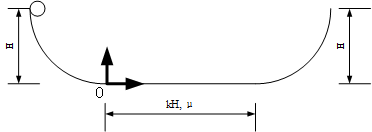
\includegraphics[width=0.5\textwidth]{../../resources/T0001.png}
    \caption{正则项的几何意义}
    \label{fig:1}
\end{figure*}


%%============
%%  ** Author: Shepherd Qirong
%%  ** Date: 2019-08-10 19:42:00
%%  ** Github: https://github.com/ShepherdQR
%%  ** LastEditors: Shepherd Qirong
%%  ** LastEditTime: 2021-12-20 23:45:13
%%  ** Copyright (c) 2019--20xx Shepherd Qirong. All rights reserved.
%%============

\chapter{Topology}

\section{AlgebraicTopology}
\subsection{摘要}
拓扑空间概念、性质、构造方法(如映射锥)
基本群的计算方法
奇异同调群3个定理:同伦不变性,正合序列,切除定理
奇异上同调(有环结构),泛系数定理,K\H unneth定理
代数拓扑通过寻找拓扑不变量给拓扑空间做分类。通过函子,把输入的拓扑空间变成群,把映射对应为同态,把同胚对应为同构。梦想是通过证明同构能够断言空间同胚。梦想还未实现,目前三维流形的分类为完成。
\subsection{拓扑空间}
通常研究连续映射、度量空间\\
性质:紧致性(任意开覆盖有子覆盖),连通性(不能表示成不相交的开子集之并),道路连通,分离性\\
同胚:对于对于拓扑空间X和Y,称$X\cong Y$,如果对于$ X \autorightleftharpoons{f}{g}Y $,有$ g\circ f =1_X,f\circ g=1_Y $\\
拓扑性质:同胚意义下不变的性质















 
\begin{comment}
    dsa 
    X \autorightleftharpoons{d969696}{3}Y
    \overset{f}{ \underset{g}{\rightleftharpoons} } 
    \xlongequal[d]{dfafdsf}
    \autorightleftharpoons{f}{g} Z

    \begin{equation}
    \label{homeomorphism}
    \begin{split}
        &\text{if: }X \autorightleftharpoons{f}{g}Y\\
        &\text{where: }g\circ f =1_X,f\circ g=1_Y\\
        &\text{then: }X\cong Y\\
    \end{split}
    \end{equation}

\end{comment}


%%============
%%  ** Author: Shepherd Qirong
%%  ** Date: 2019-06-10 18:32:30
%%  ** Github: https://github.com/ShepherdQR
%%  ** LastEditors: Shepherd Qirong
%%  ** LastEditTime: 2021-12-20 23:53:26
%%  ** Copyright (c) 2019--20xx Shepherd Qirong. All rights reserved.
%%============
\chapter{GroupTheory}

\chapter{GroupRepresentation}

\section{Introduction}
丘维声。\\
运算:笛卡尔积$S \times S \mapsto S$是集合S的二元代数运算。现代数学的鲜明特征是研究有各种运算的集合,称为代数系统。\\
现代数学的两大特征,1)研究代数系统的结构;2)利用同态映射研究代数系统结构。\\
核心:群表示论是研究G到各个线性空间的可逆线性变换群的各种同态映射,以获得G结构的完整信息。\\
群表示论是研究群结构的最强有力的工具。应用如晶体学,量子力学,抽象调和分析,组合数学,密码学,纠错编码\\
必备参考书,《抽象代数基础》丘维声,高教出版社,《高等代数学习指导书 下》丘维声,清华大学。

\subsection{环,域,群}

\begin{table}[htbp]
\newcommand{\tabincell}[2]{\begin{tabular}{@{}#1@{}}#2\end
{tabular}}
\centering
  \caption{algebra system }
  \label{tab:label}
    \begin{tabular}{cccc}
    \toprule
    名称 & 运算 & 性质 & 举例\\
    \midrule
    \multirow{2}{*}{ring}&  加法;& 交换,结合,0元,负元;&\multirow{2}{*}{\tabincell{c}{整数集$\mathbb Z$,偶数集$2\mathbb Z$,\\一元实系数多项式$\mathbb R(x)$,实n阶矩阵$M_n(\mathbb R)$}}\\
    & 乘法 & 结合,左右分配律 & \\
    \bottomrule
    \end{tabular}
\end{table}
交换环,乘法可交换。单位元。\\
例子,星期i,记为$\bar i =\left\{ 7k+i \right\} |k\in \mathbb Z$,收集起$\bar i$可以实现整数的划分。类似的,定义模m剩余类:
\begin{equation}
    \mathbb Z_m =\left\{ \bar i | i=1, \cdots ,m-1 \right\}
\end{equation}
定义加法和乘法,有模m剩余类环
\begin{equation}
\begin{split}
&\bar i + \bar j =\bar{i+j}\\
& \bar i \cdot \bar j = \bar{i \cdot j}
\end{split}
\end{equation}
可逆元,单位a:$a \in  ring R, \exists b \in R, ab=ba=e$\\
左零因子a:$a \neq 0, \exists c \neq 0,ac=0$\\
例子:$\mathbb Z_8$,零因子2,4,6;可逆元3,5,7;\\
例子:$\mathbb Z_7$,每个非零元都可逆;\\

域F:有单位元e的环,且每个非零元都可逆。
例子:有理数集,实数集,复数集$\mathbb {Q,R,Z}$\\
域F中可以定义除法。

群G:只有乘法,结合律,单位元,每个元素有逆元。\\
例子:$\mathbb Z_m^*$ :$\mathbb Z_m$所有可逆元的集合,发现只对乘法封闭,称为Zm的单位群;如域F上的所有可逆矩阵的集合$Gl_n(\mathbb F)$,只有乘法,称为域$\mathbb F$上的一般线性群。\\
阿贝尔群:乘法可交换。\\
例子:$GL(V)$,域F上的线性空间V的所有可逆线性变换,对于映射的乘法行程的V上可逆线性变换群。
子群:H<G\\

\subsection{等价关系与左陪集}
研究G的第一个途径:利用子群H研究G.\\
集合的划分与等价关系。对于$a,b \in G$,定义 $a~b:\Leftrightarrow b^{-1}a \in H$,易有关系~具有反射性(e在H中),对称性,传递性,所以这是等价关系。\\
定义a的等价类:
\begin{equation}
\begin{split}
\bar a  & :=\left\{ x \in G |x~a \right\}\\
        &:=\left\{ x \in G | a^{-1}x \in H \right\}\\
        &= \left\{ x\in G | x=ah,h\in H \right\}\\
        & =\left\{ ah |h \in H \right\}\\
        &=:aH
\end{split}
\end{equation}
aH称为以a为代表的H的一个左陪集,是一个等价类。\\
根据等价类的性质,有1)$aH=bH \Leftrightarrow b^{-1}a \in H$;2) aH与bH或者相等,或者不相交(交集为空集)。所以 H的所有左陪集给出G的一个划分,记为$G/H$,称为G关于H的左商集。G/H的基数称为G关于H的指数,记为[G:H]。基数相同可建立双射。\\
G关于H的左陪集分解:$[G:H]=r, G=eH \bigcup a_1H \bigcup \cdots \bigcup a_{r-1}H$。\\
拉格朗日定理:对于有限群G,易有其元素个数$|G|=|H|[G:H]$,即任何子群的阶是群的阶的因数。推论:1)n阶群G的任意元素a,有$a^n \in G$;2)素数阶群是循环群。

\subsection{同态}
研究G的第二个途径:通过研究G到G'的保持运算的映射,同态映射,简称同态。同态要变,是函数。\\
通常利用G到$\Omega$的同态,等价于G在$\Omega$的作用。既可以研究G的结构,又可以对$\Omega$的性质有了解\\
$S(\Omega)$:$\Omega$的全变换群,Full Transformation Group on Set $\Omega$, $\Omega$自身的所有双射组成的集合,对于映射的乘法构成的一个群.\\

\subsection{作业}
1.环R中,0a=a0=0 \\
2.有e的环中,零因子不是可逆元\\
3.$\mathbb Z_m$中每个元素要么是可逆元要么是零因子;\\
4. $M_n(\mathbb F)$中,每个矩阵是可逆矩阵或者是零因子。

\section{Abel群的表示}
\subsection{映射}
映射:$f:a \mapsto b \Leftrightarrow f(a)=b$,原象,象。映射f的定义域(domain)A,陪域(codomain)B。映射得到的所有象的集合叫值域,记作$f(A)$,或Imf。\\
满射,onto,到上:$f(A)=B$\\
单射,一一的,每个a对应的b是不同的。\\
双射,两个集合一一对应。\\
逆映射。对于$f:A \to B, g: B \to A$,有$g \circ f =1_A, f \circ g =1_B$。可逆的f是双射。\\

线性映射、线性变换是线性空间的同态映射,有点乘和加法。\\
补空间:域$\mathbb F$上的线性空间U<V,则$\exists W, V=U \oplus W$。对于实内积空间V,U是有限维的,$W=U^{\perp}$,正交补空间,唯一的。\\
投影变换:域$\mathbb F$上的线性空间$V=U \oplus W$,有$\mathbf \alpha =\mathbf \alpha _U+\mathbf \alpha _W$, 有投影变换$P_U:\mathbf \alpha \mapsto \mathbf \alpha _U$.投影变换保持加法和数乘,是V上的线性变换。投影是同态映射。\\
几何空间:以原点O为起点的定位向量组成的实线性空间。知道一空间点在两个坐标面的投影坐标可完全确定点。

\subsection{群的同态}
同态映射:G到G'的映射$\sigma: \sigma(a,b)=\sigma(a) \sigma(b)$。单射的话是单同态。满射是满同态。双射是同构,此时两个群同构,$G \cong G'$。\\
同态的性质:1)单位元、逆元、子群映射过去是G’的单位元、逆元、子群。例如$G<G \Rightarrow \sigma(G)=Im\sigma <G'$,同态的像是G'的子群\\
刻化单同态:找到映射成单位元的原象,定义同态的核,$Ker\sigma:=\left\{ a \in G | \sigma(a)=e' \right\}$.易有同态的核是G的子群。对于单同态,$Ker\sigma=\left\{ e \right\}$.\\
子集乘法:类似与点乘,a的所有和b的所有的乘积方式的组合。乘法满足结合律。\\

\subsection{正规子群}
$ \forall k \in \ker \sigma, \forall g\in G$, we have:
\begin{equation}
\begin{split}
&\sigma(gkg^{-1})=\sigma(g)\sigma(k)\sigma(g^{-1})=e'\\
& \therefore gkg^{-1}\in \ker \sigma\\
& \therefore g \ker \sigma g^{-1} \subset \ker \sigma\\
& \& \ g^{-1}  \ker \sigma g\subset \ker \sigma\\
& \therefore g \ker \sigma g^{-1}=\ker \sigma\\
\end{split}
\end{equation}
normal subgroup正规子群:$H \lhd G :\forall g \in G, gHg^{-1}=H$, $gHg^{-1}$是g的共轭子群。\\
性质:$H \lhd G \Leftrightarrow gHg^{-1}=H,\forall g \in G \Leftrightarrow gH=Hg$,H的左右陪集相等;\\
G关于正规子群H的商群:规定正规子群H的商群G/H乘法:$(aH)(bH)=abH$\\
\subsection{群同态基本定理}
\begin{equation}
\begin{split}
\psi : &G/ \ker \sigma \to Im \sigma\\
& a (\ker \sigma) \mapsto \sigma(a)
\end{split}
\end{equation}
看映射$\psi$的性质:
\begin{equation}
\label{证明同构1}
\left.
\begin{aligned}
& a(\ker \sigma)=b(\ker \sigma)\\
& \Leftrightarrow b^{-1}a \in \ker \sigma\\
&\sigma(b^{-1}a)=e'\\
&\therefore \sigma(a)=\sigma(b)
\end{aligned}
\right\} \Rightarrow \psi \ is \ surjection\\
\end{equation}
从是映射、是单射、是满的,得到是双射;\\
Let $K=\ker \sigma$, $\psi [(aK)(bK)]=\psi (abK)=\sigma(ab)=\psi(aK)\psi(bK)$,所以保持运算,所以是同构,所以$G/ \ker \sigma \cong Im \sigma$\\
群同态基本定理:$\ker \sigma \lhd G \ \& \   G/ \ker \sigma \cong Im \sigma  $ 



\section{线性表示}
$GL(V)$: 对于群G,域$\mathbb K$上的线性空间V,G到V的所有可逆线性变换的集合,对于映射的乘法成为一个可逆线性变换群。\\
G到GL(V)的同态$\psi $ 是G在$\mathbb K$ 上的线性表示,简称为$\mathbb K$ 表示,或者简称为表示。\\
V叫做表示空间,表示次数$\deg \psi := \dim V$\\
$(\psi ,V$)\\
如用两个视图可完全确定空间曲线,即做了两个同态。\\
$\ker \psi =\left\{ e_G \right\}$,$\psi $是忠实的;\\
$\ker \psi =G$, $\psi$是平凡的;|、
称一次的平凡表示$\psi $是G的主表示,单位表示,记作$1_G$;\\
$dimV=n$时,有$\psi (g)$在基$\left\{ \alpha_1,\cdots , \alpha_n \right\}$下的矩阵$\Phi(g)$是 $\mathbb K$ 上的可逆矩阵,由同构$GL(V) \cong GLn(\mathbb K)$,有G到$GLn(\mathbb K)$的同态$\Phi$,称为G在$\mathbb K$上的n次矩阵表示。\\
$\Phi $ 称为是$\psi $提供的
\subsection{表示的等价类}
等价关系:对于G的2个k表示,$(\phi,V),(\psi,W)$,$\exists$v到w的线性空间的同构$\sigma$,定义$\psi(g)\sigma =\sigma \phi (g), \forall g \in G$,这种G的所有K表示的集合$\Omega$上的二元关系,易有具有反射性,对称性,传递性,从而是等价关系。通常关注G的k表示的等价类。\\
$(\phi,V),(\psi,W)$等价,取基后的矩阵记为$\Phi (g)| \{\alpha _i, \cdots\},\Psi (g)| \{\beta _i, \cdots\}$,同构$\sigma$把V的基映射到W上的S,有$\sigma (\{\alpha , \cdots\})=\{\beta, \cdots\}S$,$\therefore \Psi (g)S=S\Phi(g)$.所以G在K的2个矩阵表示$\Psi, \Phi$等价:次数一样且$\forall g \in G,\Psi =S\Phi (g)S^{-1}$. 所以群G的2个K表示$(\phi,V),(\psi,W)$等价,$\Leftrightarrow$K表示提供的矩阵表示$\Psi, \Phi$等价。
\subsection{例:1次表示}
G在K上的1次矩阵表示$\Phi: G \to \mathbb K^*$;非零元集合。映射是通用的不对定义域做要求,陪域是域的子集的映射叫函数。称为G上的K*函数,且由于同态保持运算,有$\Phi (gh)=\Phi (g)\Phi(h), \forall g,h \in G$, and $\Phi(e)=1$, where 1 is the unit of K*.所以一次表示是G到K*的保持运算的函数。

\subsection{例:实数和加法的1次实表示}
$f_a(x)=e^{ax}$ 是 $\mathbb R, +$的1次实表示。

\subsection{例:实数和加法的1次复表示}
$f_a(x)=e^{iax}$ 是 $(\mathbb R, +)$的1次实表示。
\begin{equation}
\label{fubiaohsi}
\begin{split}
f:(\mathbb R, +) &\to \mathbb C^*\\
x  &\mapsto e^{iax}\\
\end{split}
\end{equation}
 


%\begin{equation}
%\label{ji}
%\alpha P_{\alpha} =\beta P_{\beta}
%\end{equation}


\end{document}